\begin{titlepage}
\begin{center}

\includegraphics[scale=0.15]{OPAMP Apps/niser.png}
\line(1,0){400}\\
[2mm]
\begin{large}
\textbf{\huge Op-Amp as Comparator and Schmitt Trigger}\\ 
\end{large}
\line(1,0){250}\\
[5cm]
\large MAITREY SHARMA\\
\small (1911093)\\
[4.5cm]
Second Year Integrated M.Sc.\\
\textbf{School of Physical Sciences}\\
\textbf{National Institute of Science Education and Research, Bhubaneshwar}\\
\small March 3, 2021
\end{center} 
\end{titlepage}
\newpage
\section{Aim}
\begin{itemize}
    \item Study of Op-Amp as comparator
    \item Study of Op-Amp as Schmitt trigger
\end{itemize}
\section{Apparatus}
\noindent Op-Amp IC741, resistors, oscilloscope, DC voltage source, breadboard, multimeters and connecting wires.
\section{Theory}
\noindent The Op-Amp with a negative feedback loop are essentially analogue electric circuits. In \textbf{\emph{Analogue Electronics}}, we  deal with continuously varying signals. Thus the Op-Amp is a linear circuit element. But without the feedback loop, the output signal from the Op-Amp is very sensitive, as discussed in the last experiment. This property can be exploited to create a non-linear circuit. Thus we can design a circuit where the signals take two levels, that is a \textbf{\emph{Digital Electronics}} circuit. 
\par
\noindent The \textbf{\emph{Voltage Comparator}} is a device which does not use any feedback loop, and this the saturation caused by transistor biasing is the only output result. The output will be binary in nature caused by the positive and negative saturation. We can add a small modification in form of a threshold voltage which can help in changing the point of polarity change.
\begin{center}
    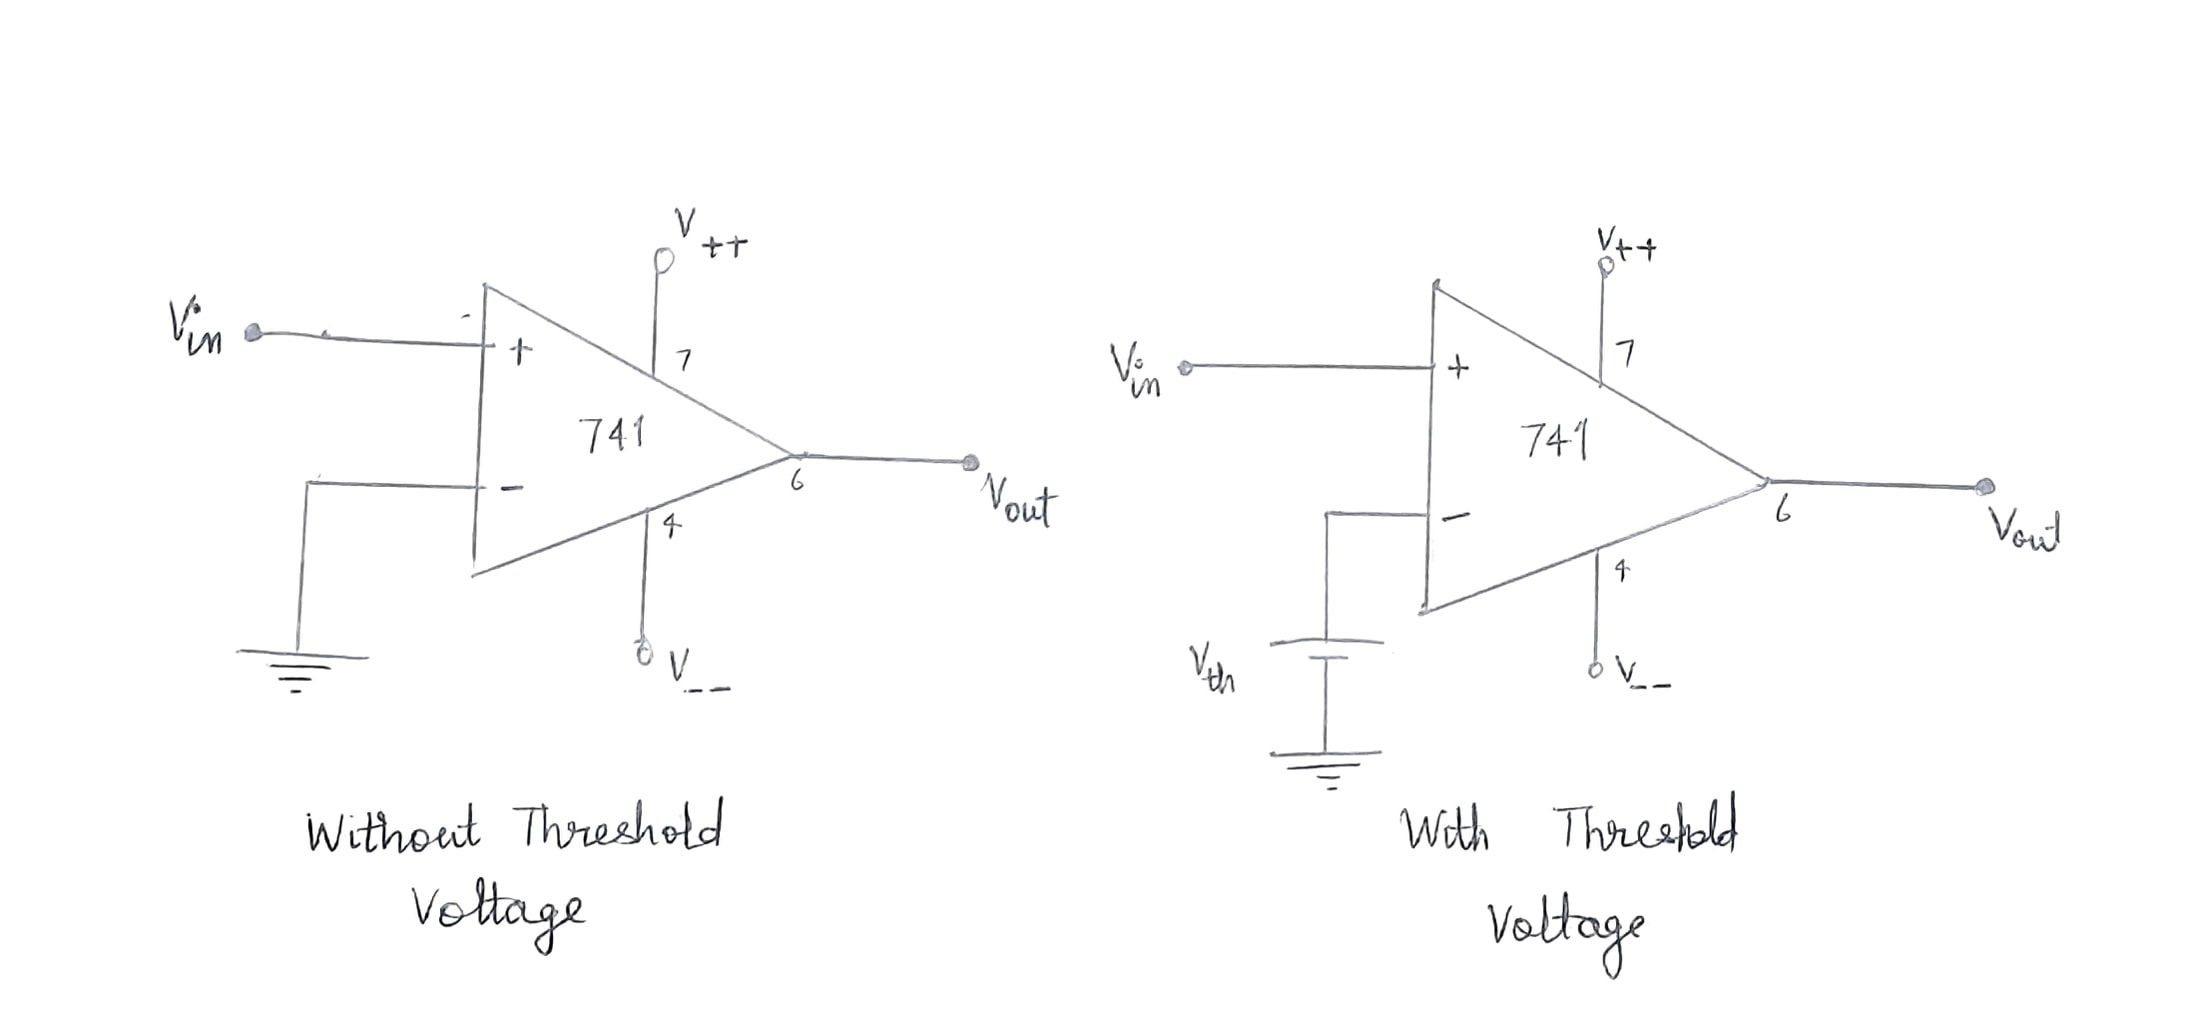
\includegraphics[scale = 0.21]{OPAMP Apps/1614500891771.jpg}
\end{center}
\begin{center}
    \textbf{Non-inverting Comparator Circuit}
\end{center}
\noindent Note that the inverting comparator can also be constructed by changing the input terminal from positive to negative. 

\noindent The \textbf{\emph{Schmitt Trigger}} is a variation of the comparator circuit which used a positive feedback to provide a toggle action. It yields a curve akin to hysteresis.
\clearpage
\begin{center}
    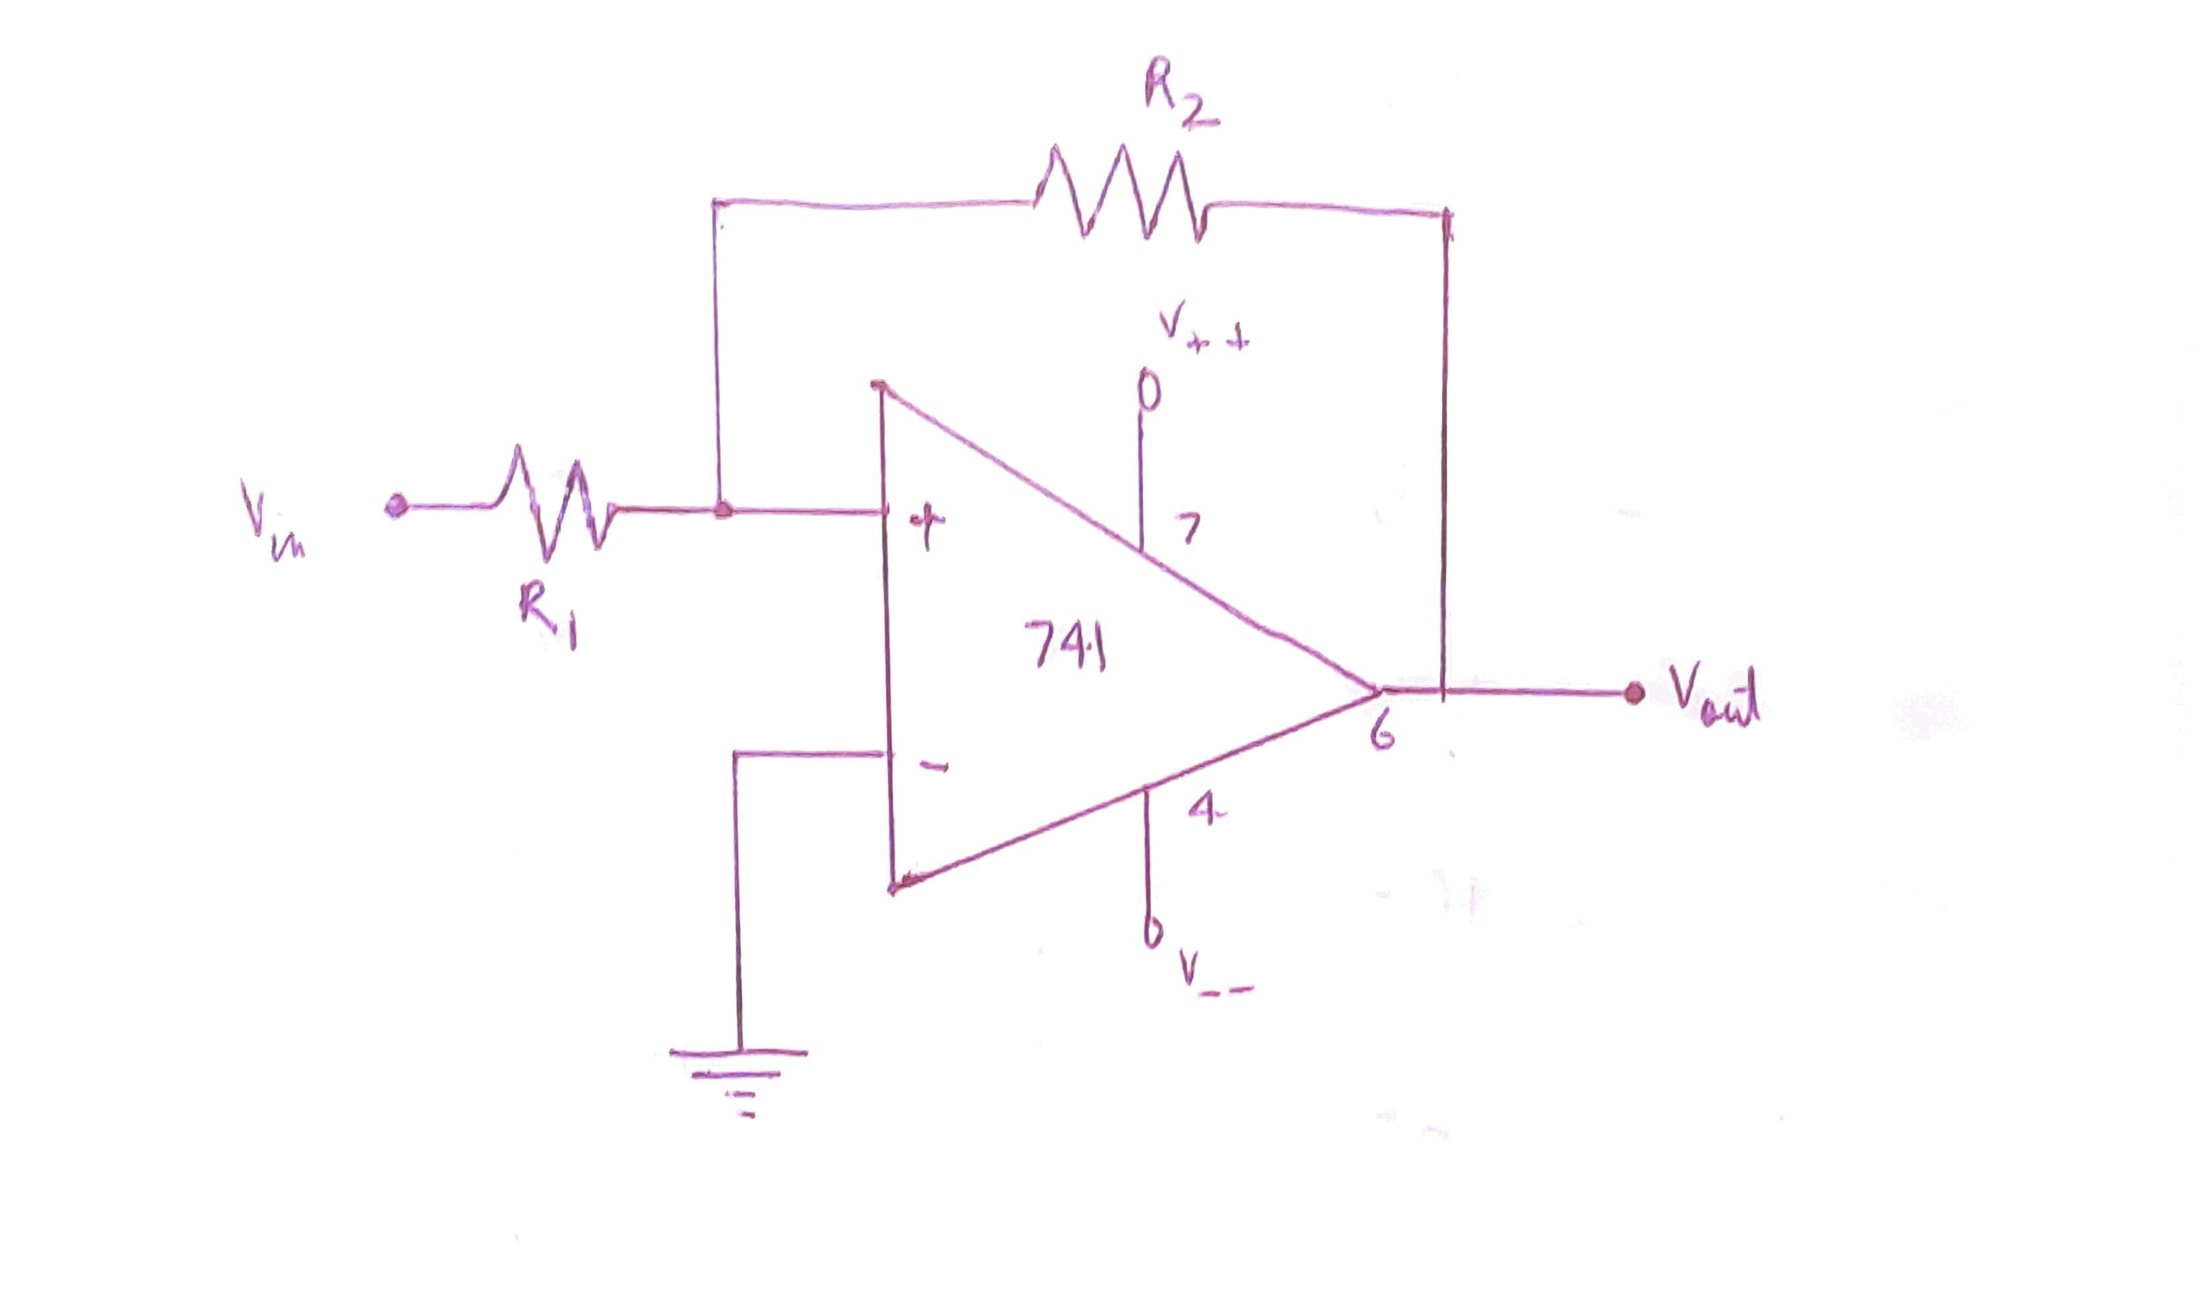
\includegraphics[scale = 0.21]{OPAMP Apps/1614500891766.jpg}
\end{center}
\begin{center}
    \textbf{Schmitt Trigger Circuit}
\end{center}

\section{Observations}
\begin{enumerate}
    \item Bias Voltage = $|V_{++}| = |V_{--}| = \SI{12}{\volt}$
    \item $V_{Th} = \SI{5.00}{\volt}$
    \item $R_1 = \SI{0.997}{k\ohm}$
    \item $R_2 = \SI{9.98}{k\ohm}$
\end{enumerate}
\clearpage
\begin{center}
    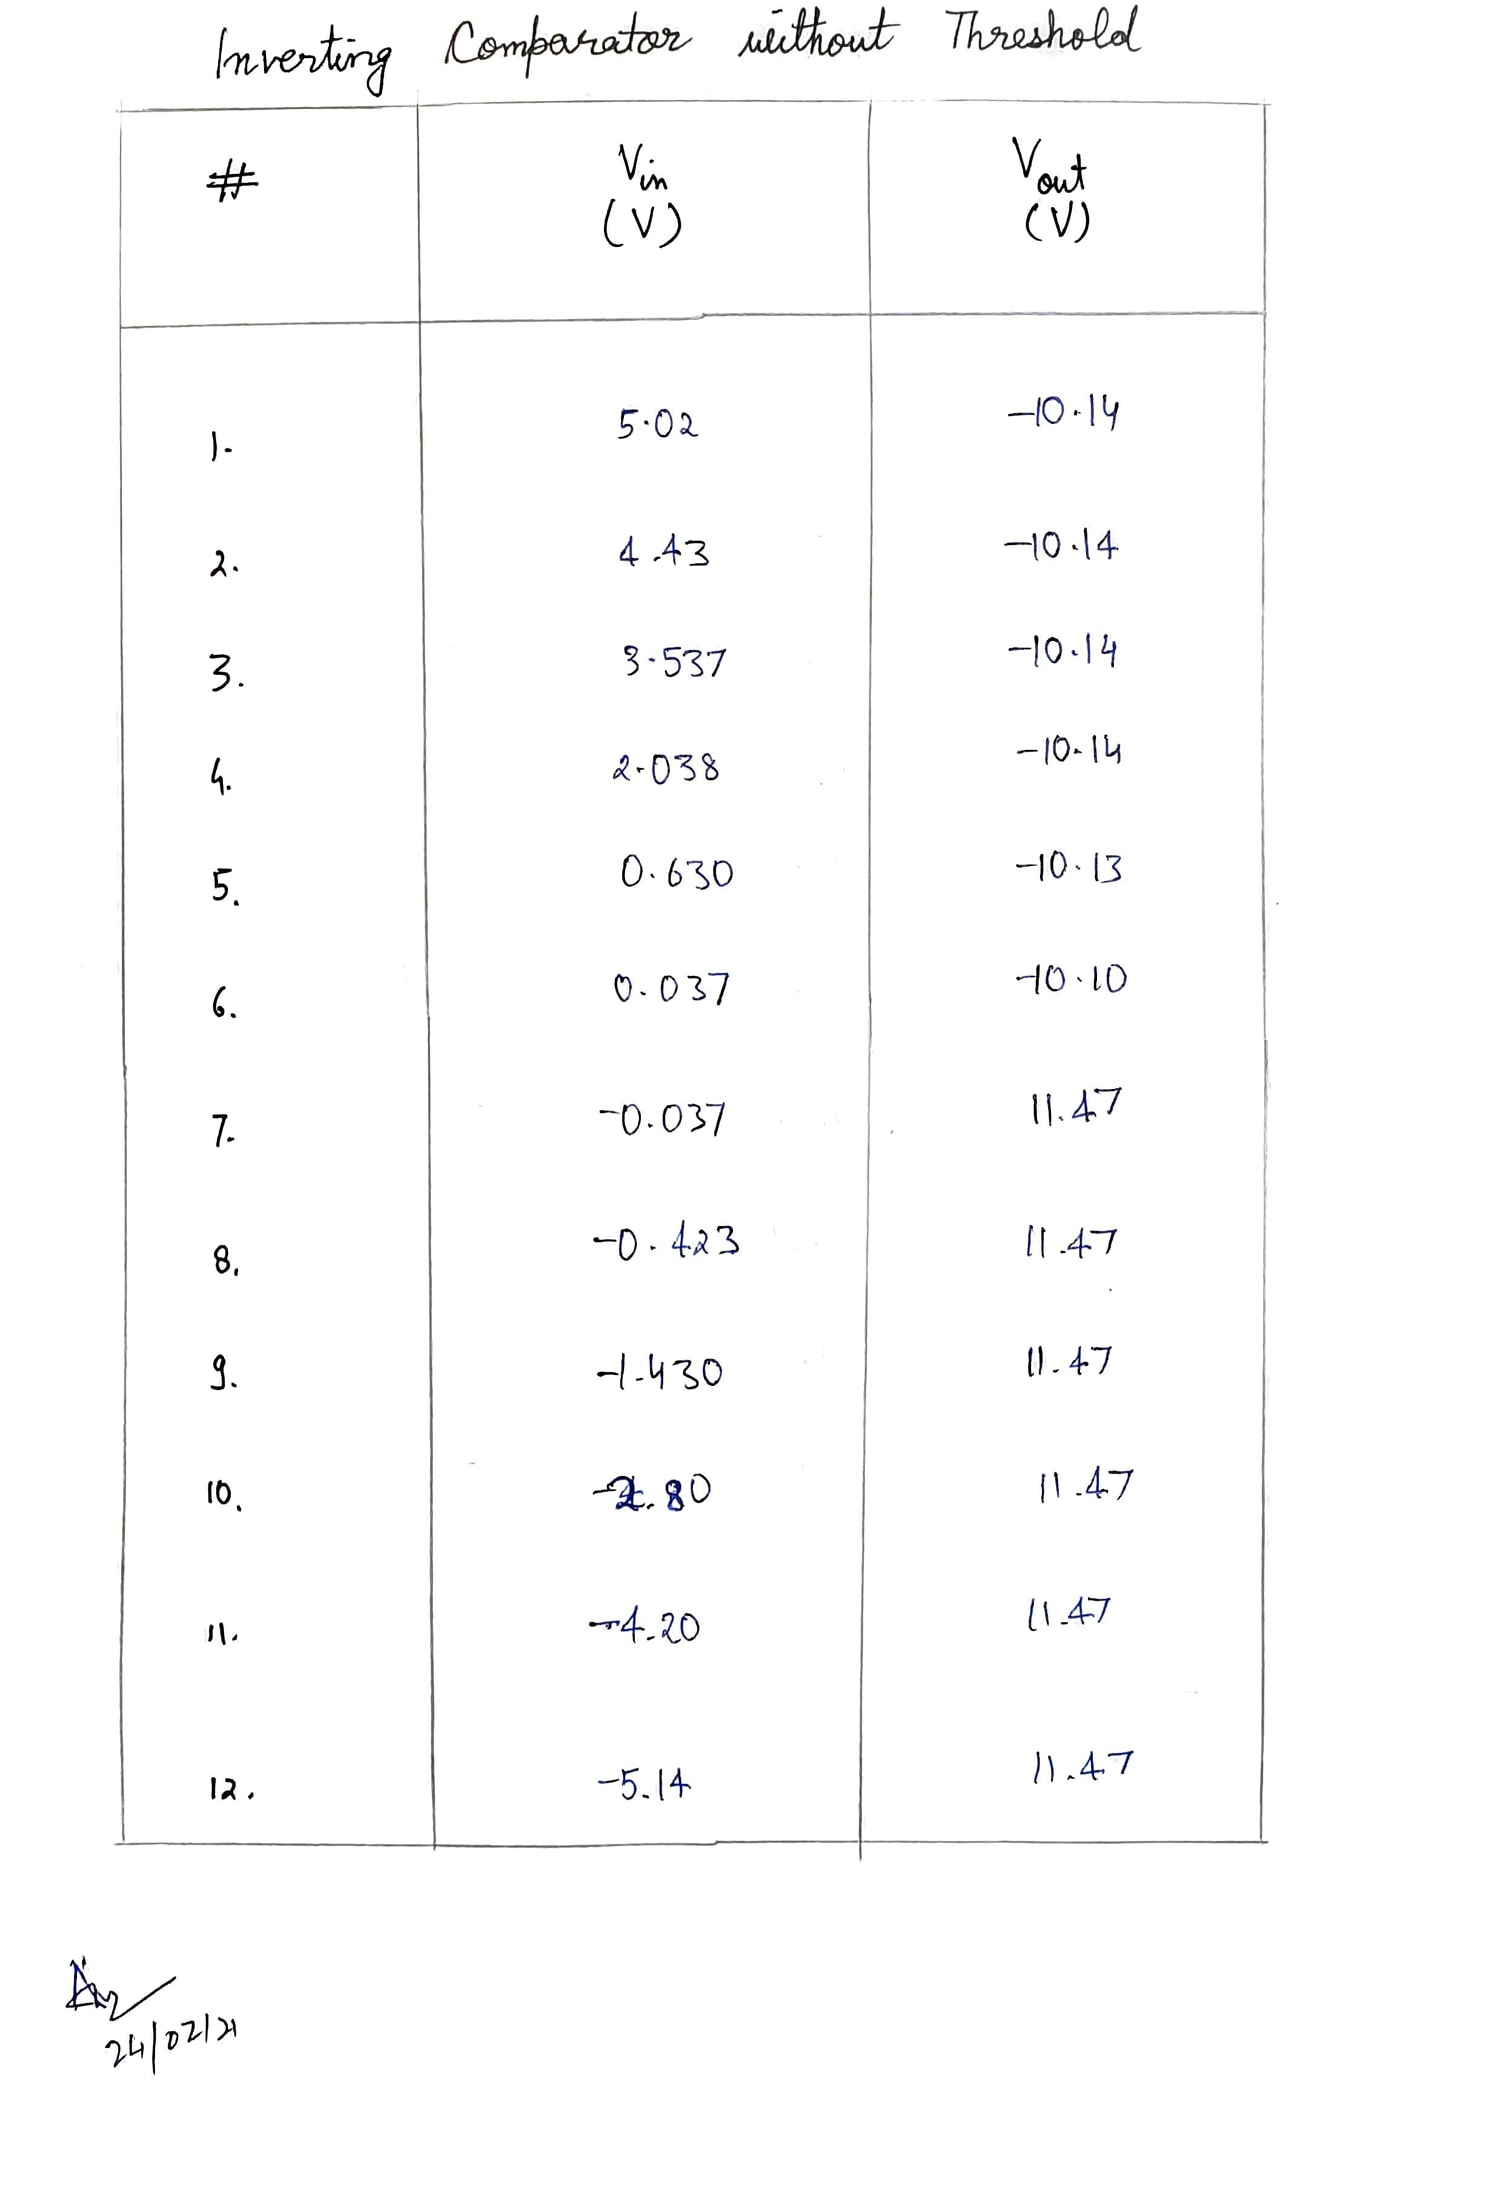
\includegraphics[scale = 0.28]{OPAMP Apps/invcomp.jpg}
\end{center}
\clearpage
\begin{center}
    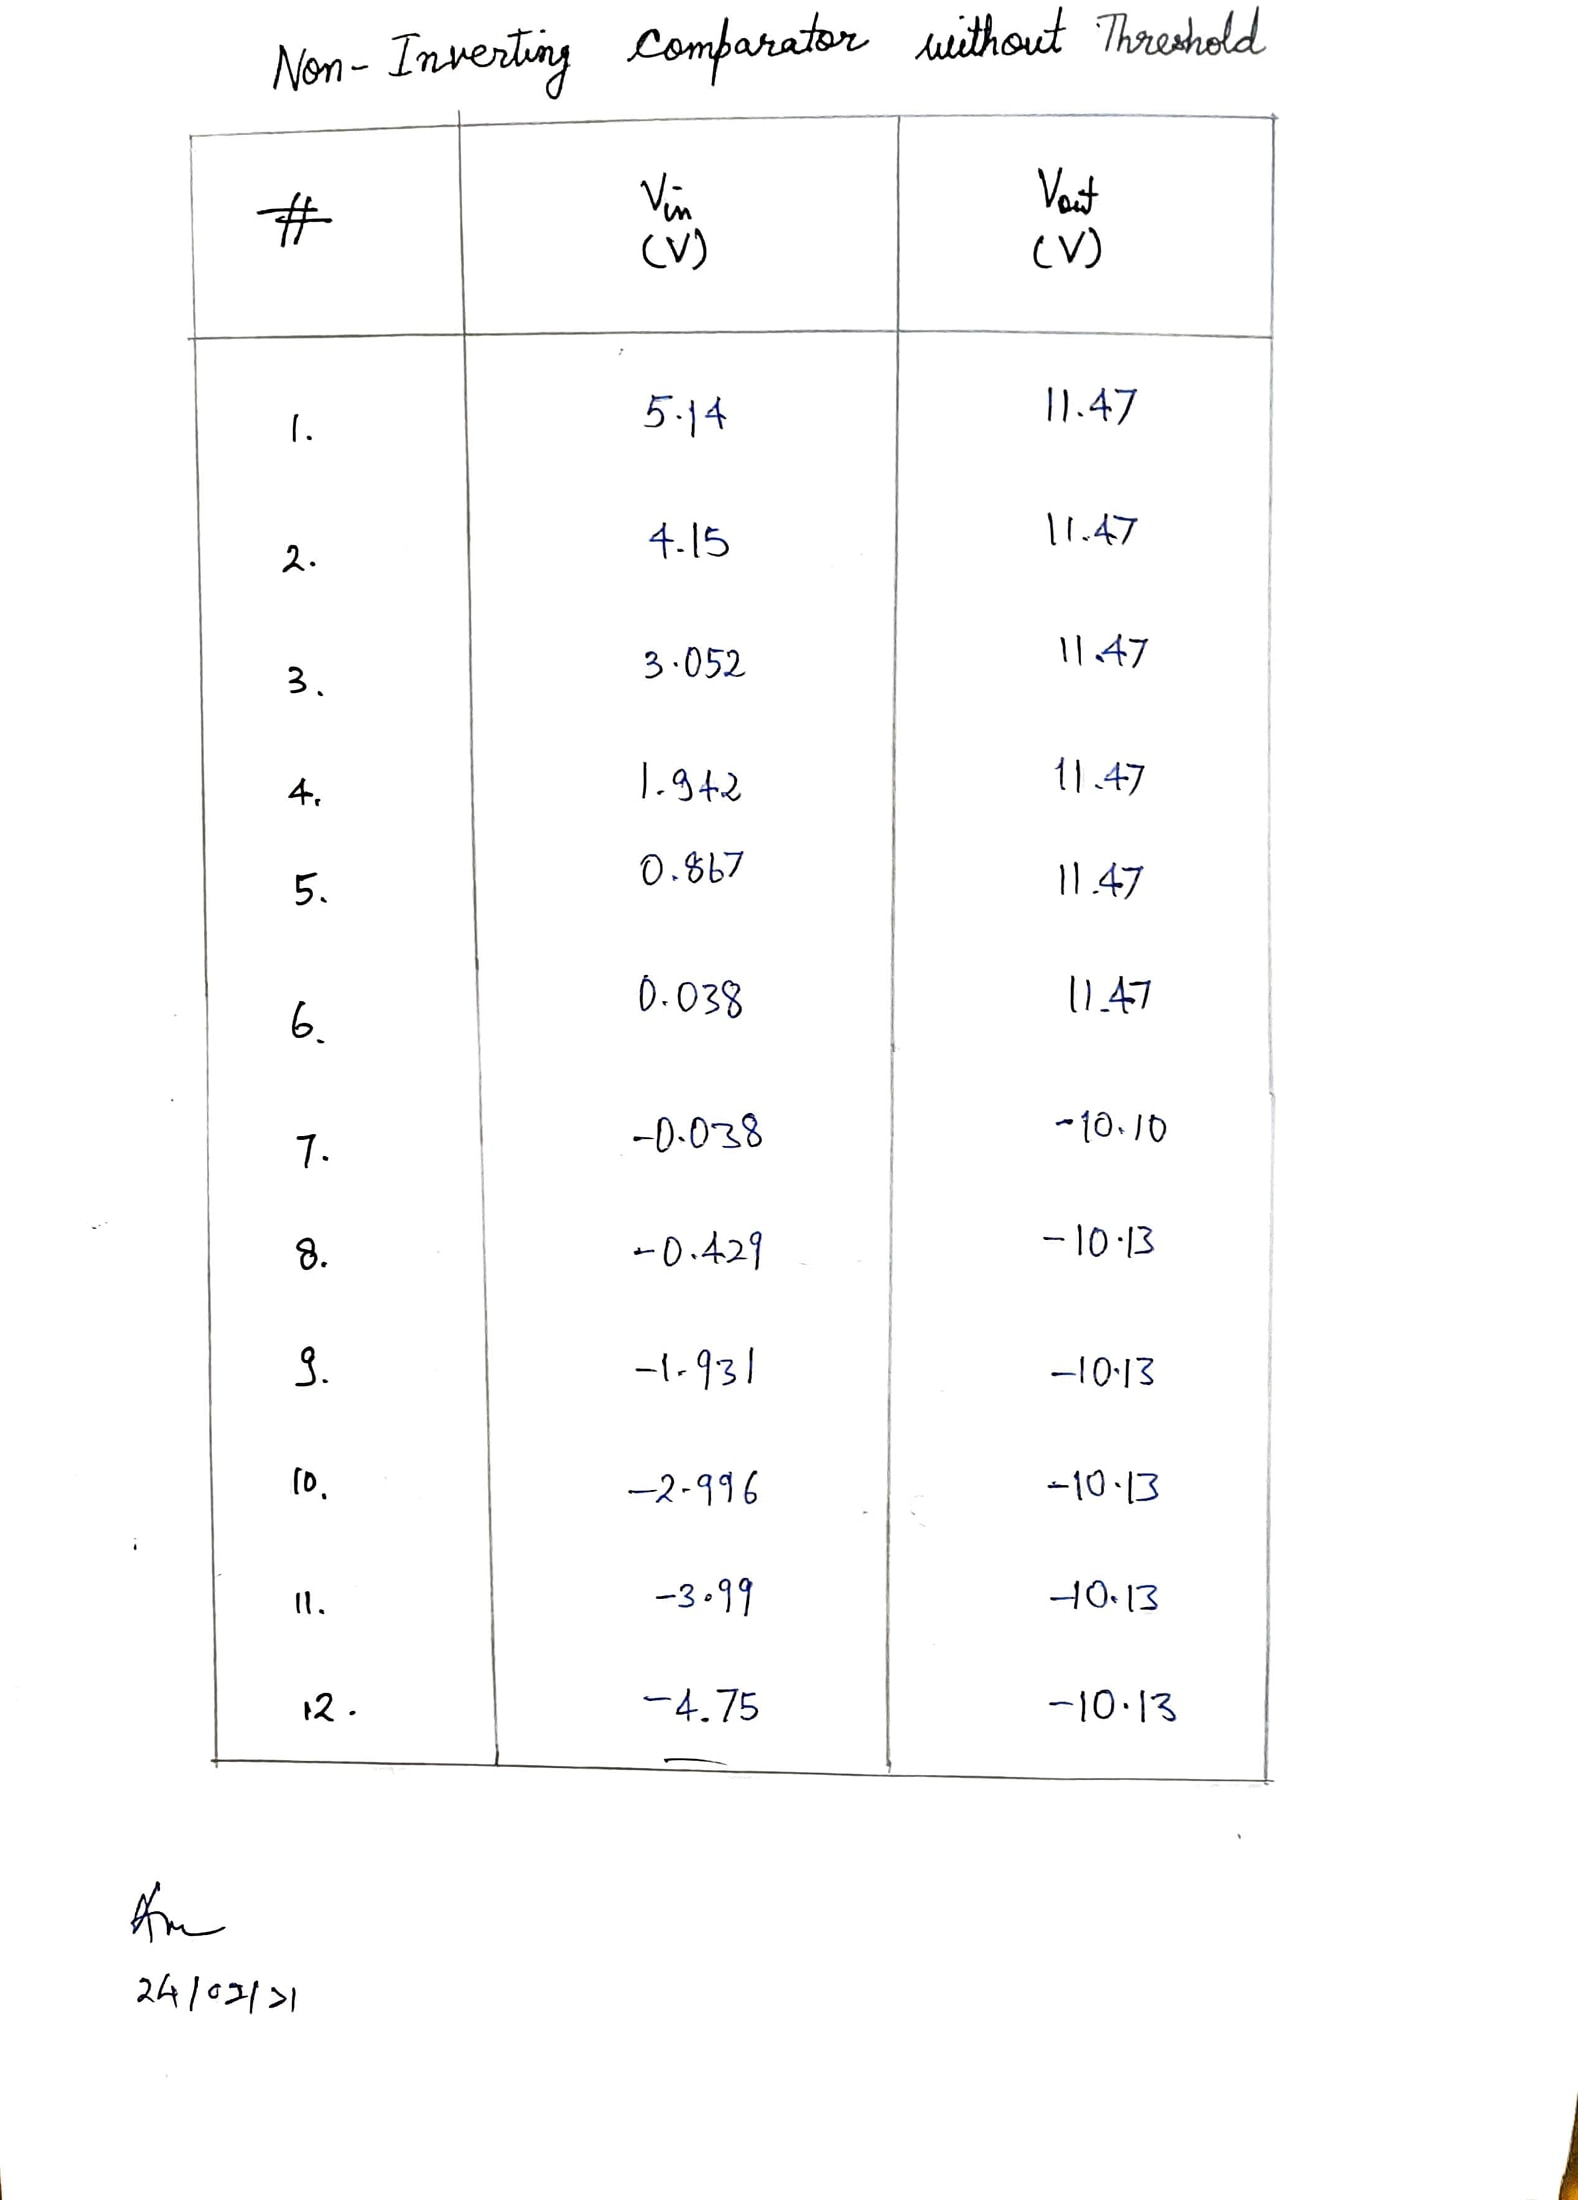
\includegraphics[scale = 0.28]{OPAMP Apps/noninvcomp.jpg}
\end{center}
\clearpage
\begin{center}
    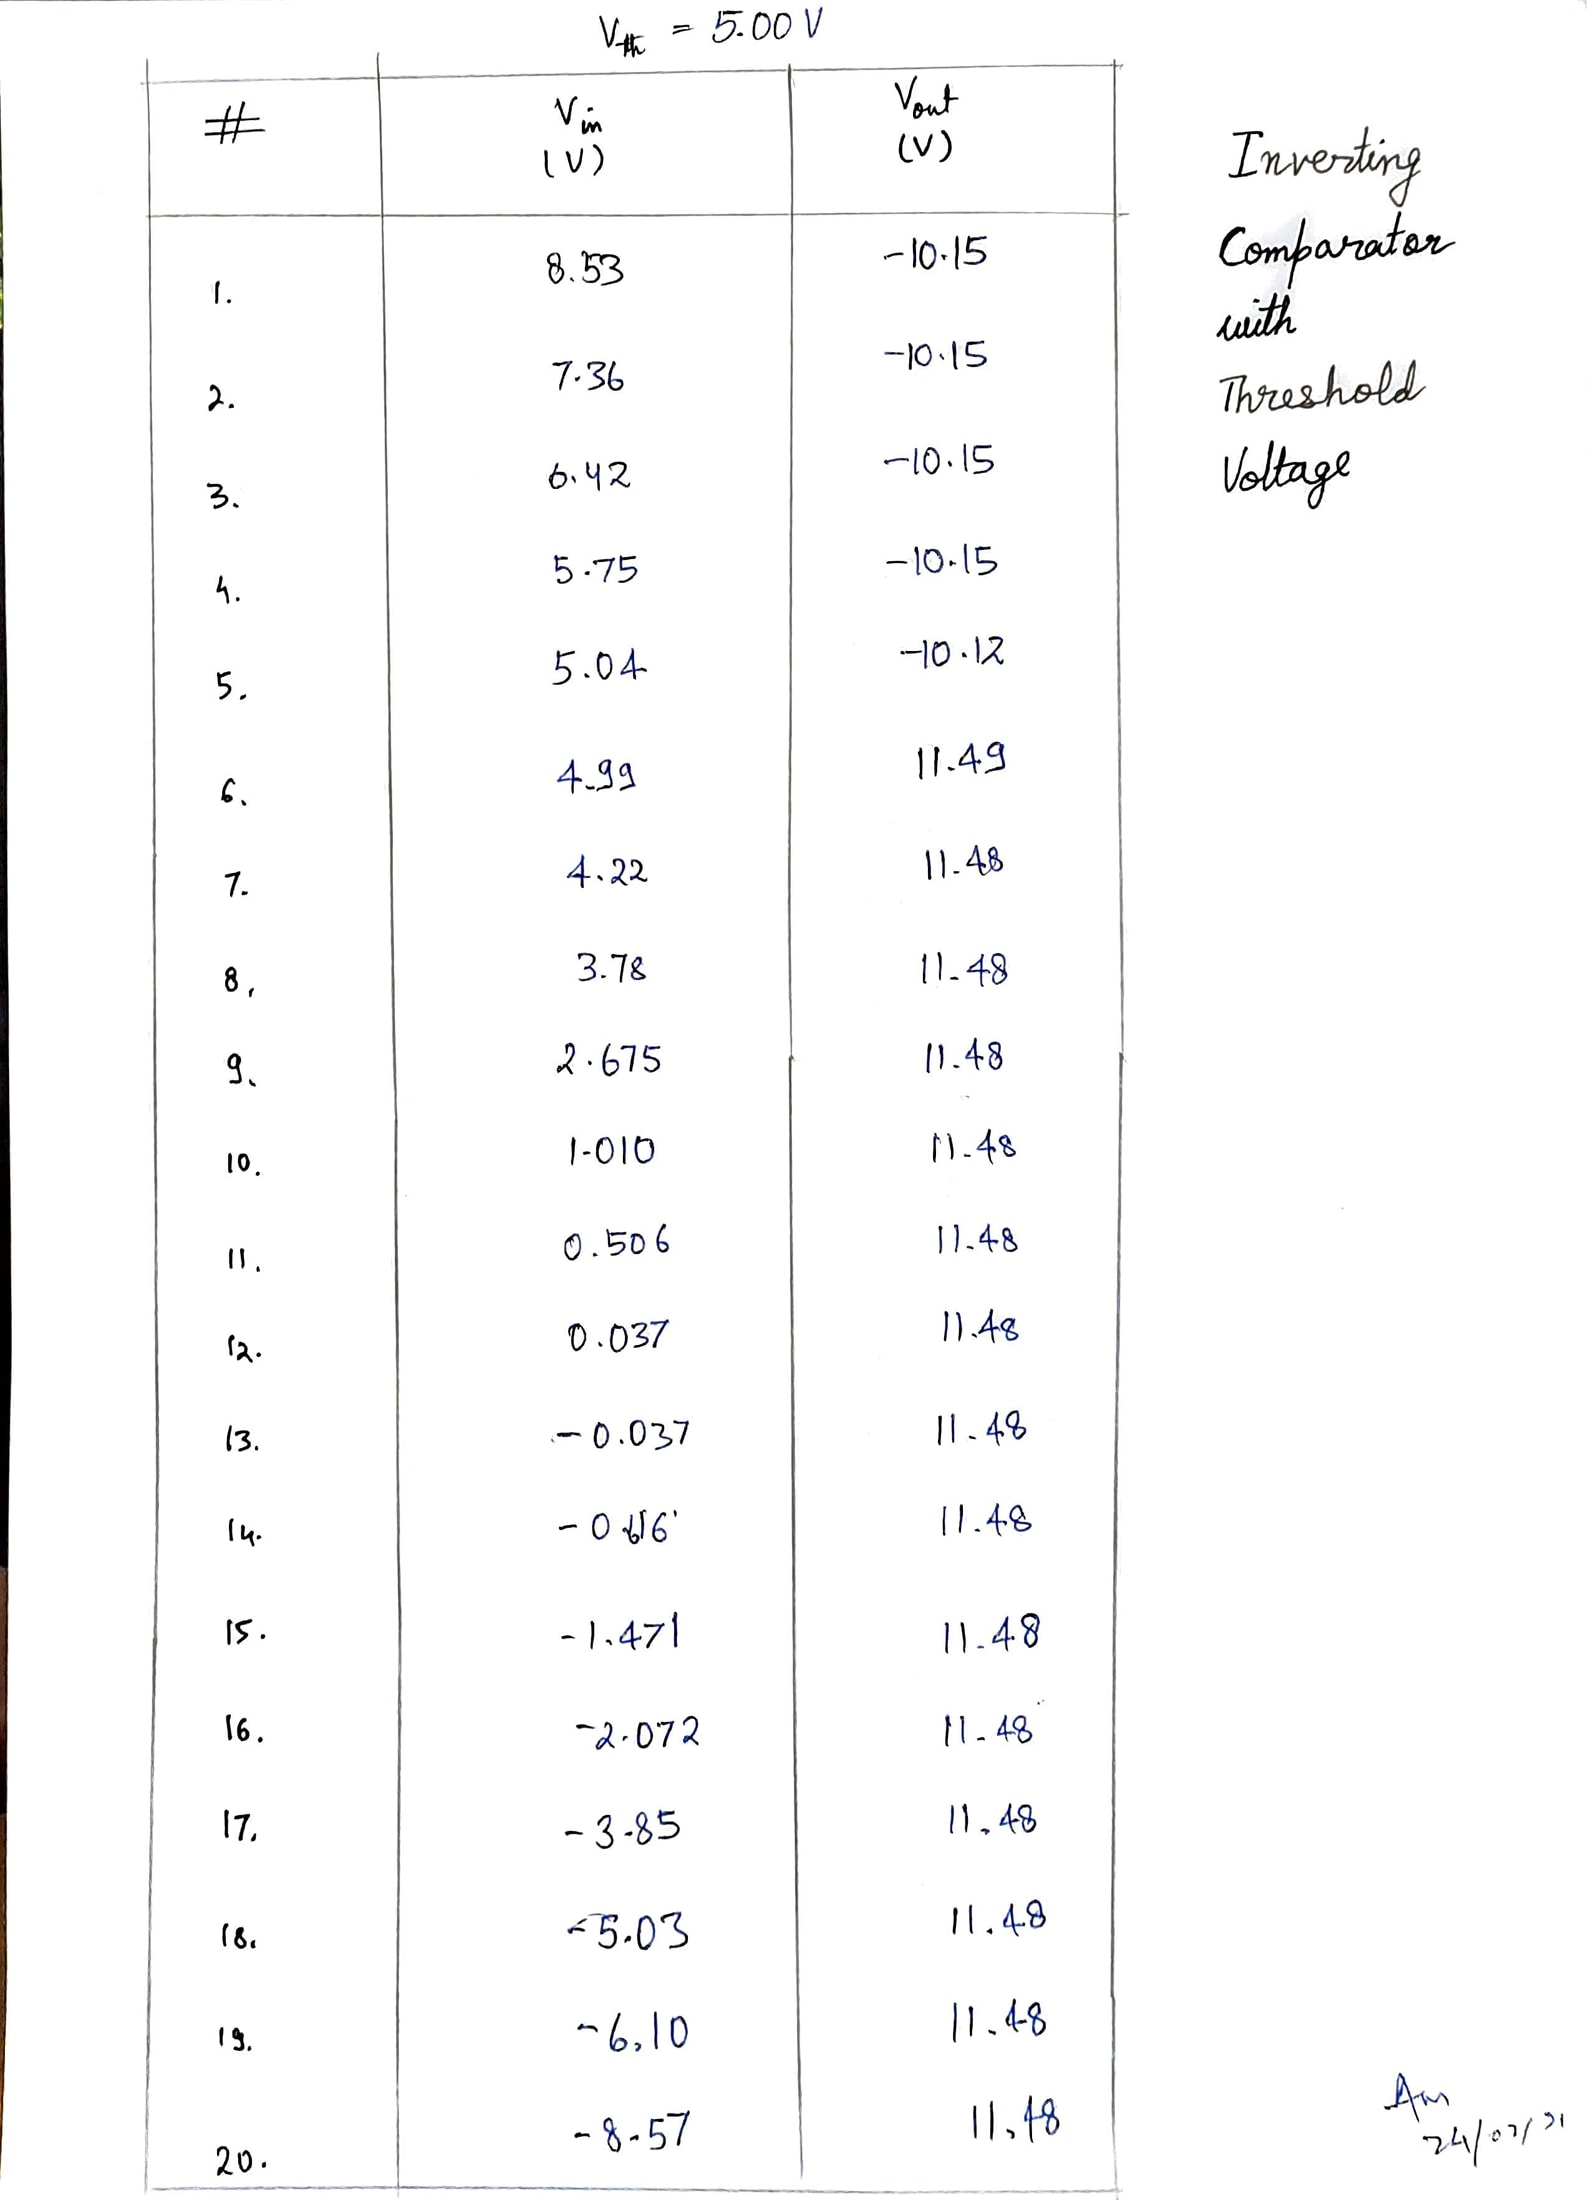
\includegraphics[scale = 0.28]{OPAMP Apps/invcompthres.jpg}
\end{center}
\clearpage
\begin{center}
    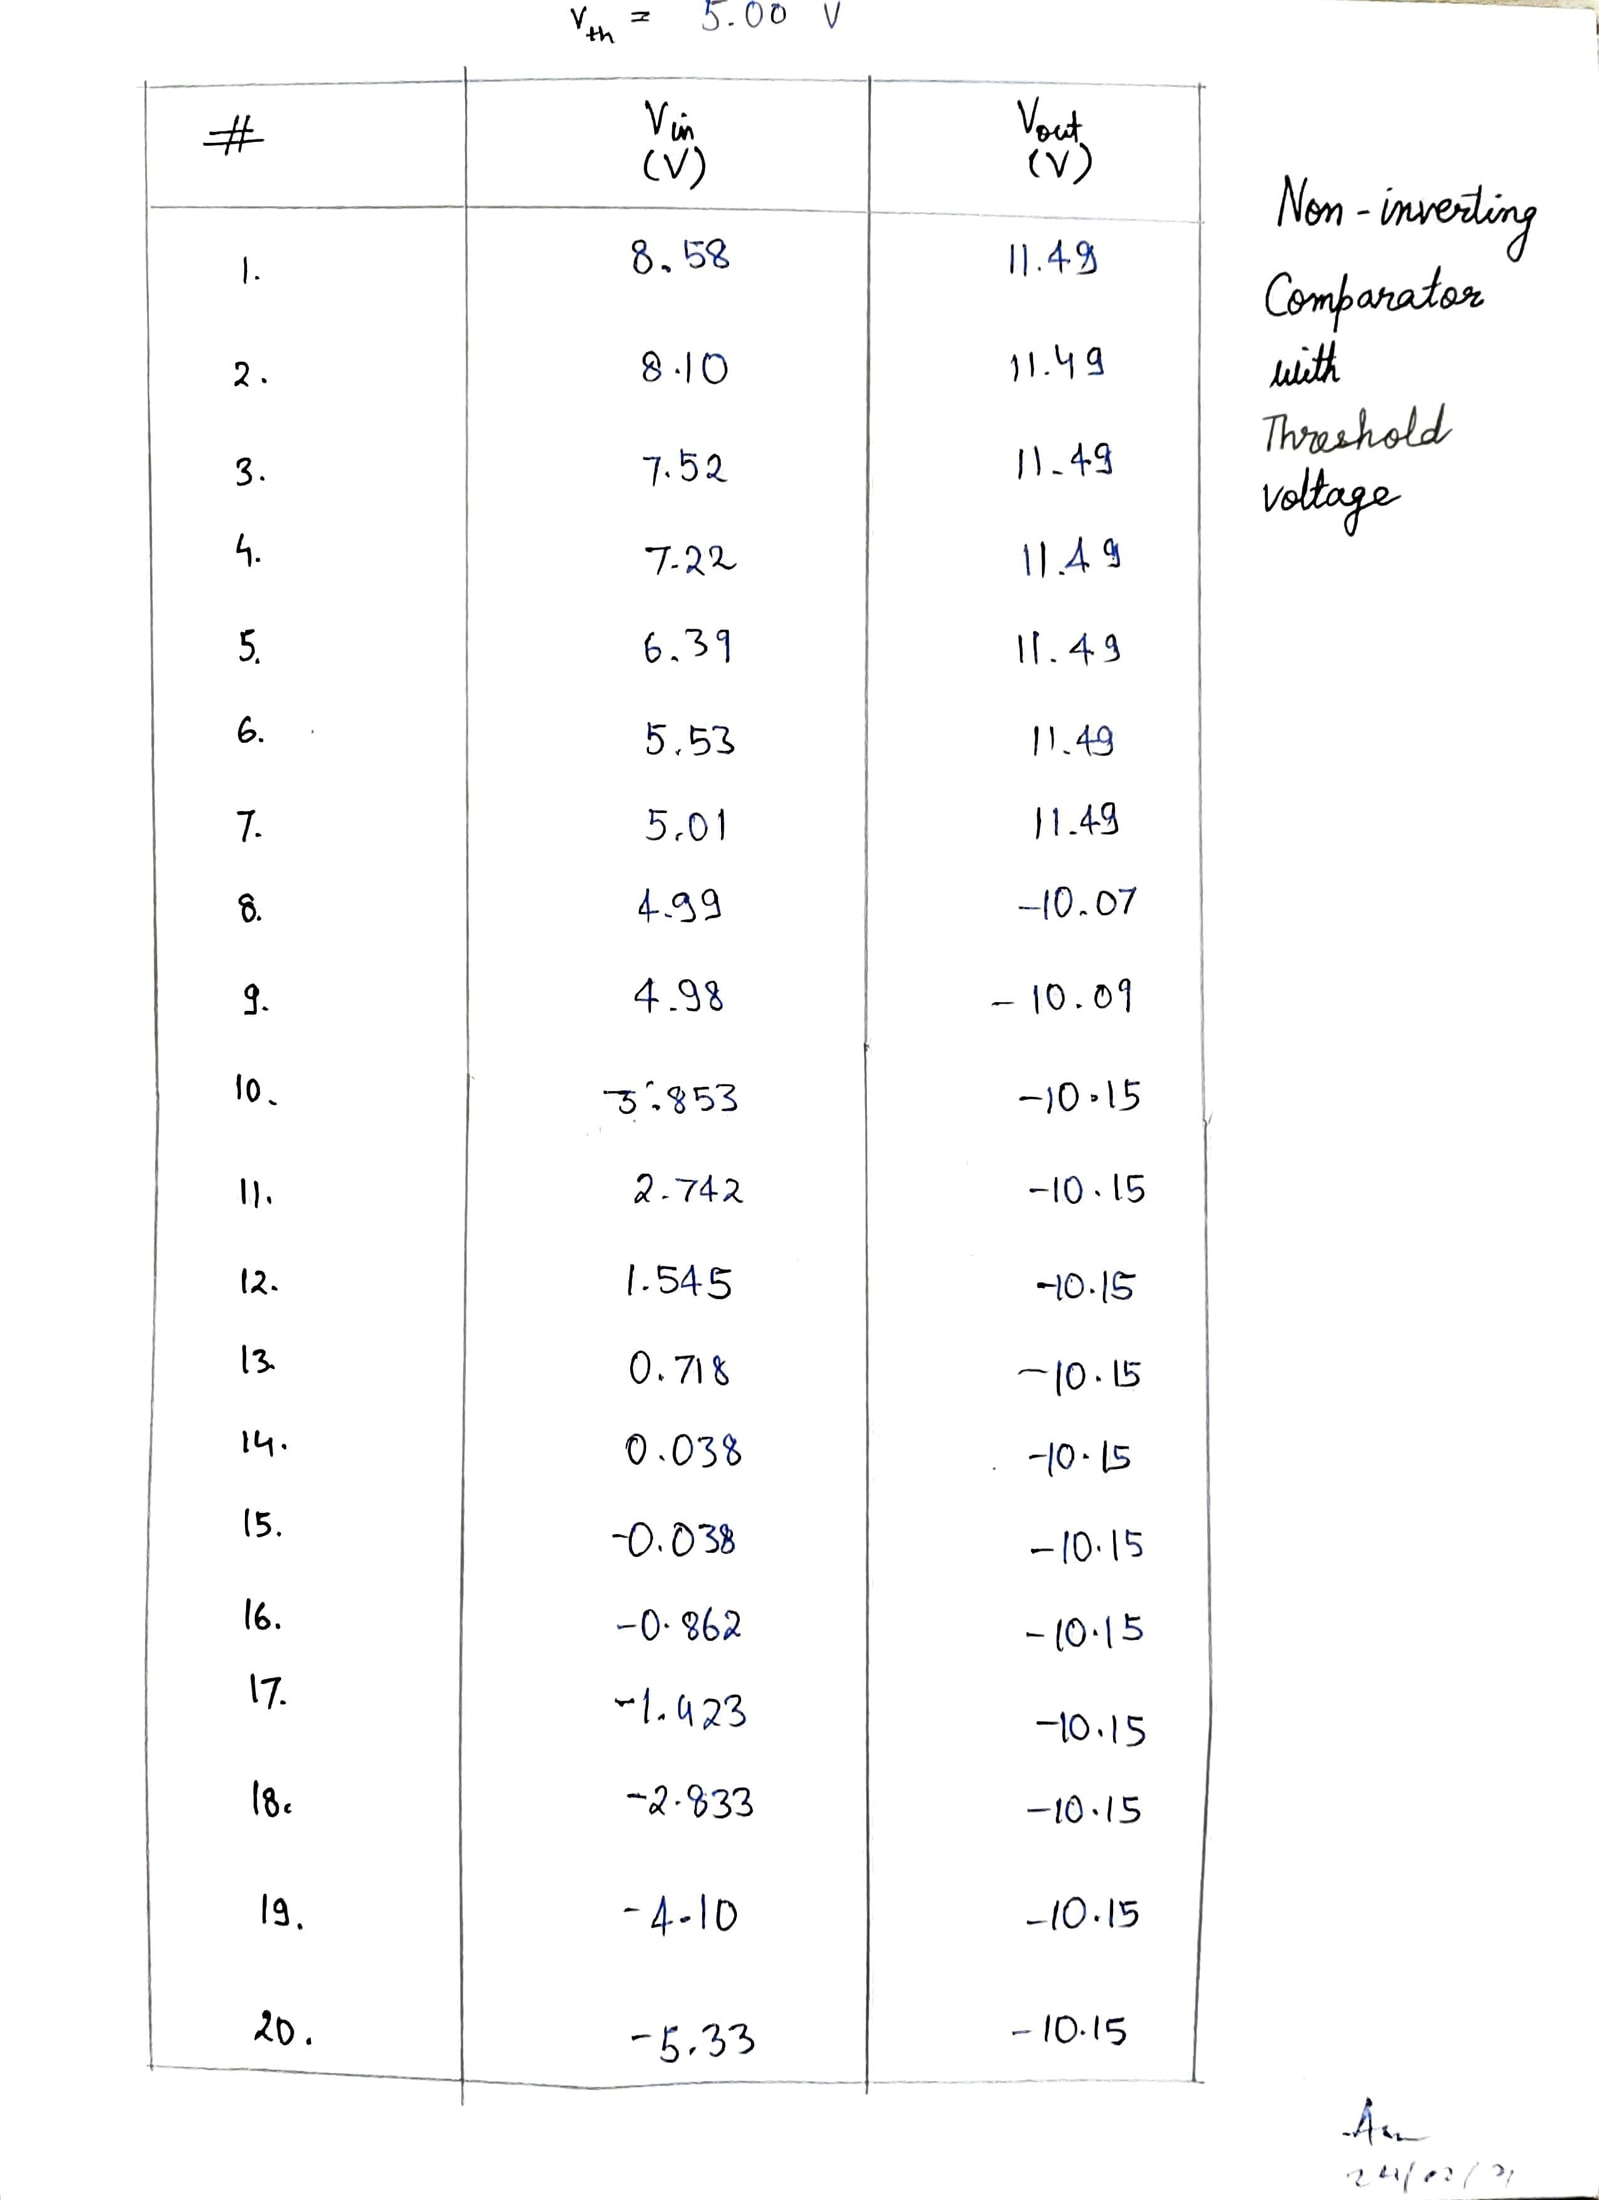
\includegraphics[scale = 0.28]{OPAMP Apps/noinvcompthres.jpg}
\end{center}
\clearpage
\section{Graphs}
\begin{center}
    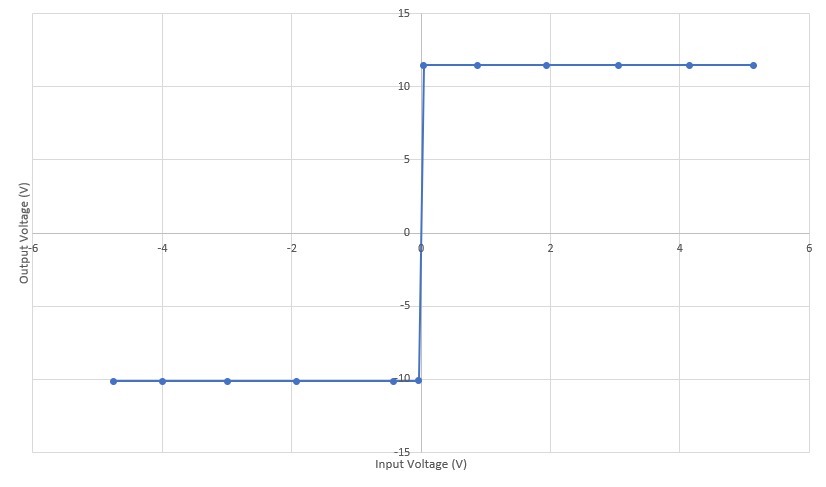
\includegraphics[scale = 0.7]{OPAMP Apps/noninvwothres.png}
\end{center}
\begin{center}
    \textbf{Non-inverting Without Threshold}
\end{center}
\begin{center}
    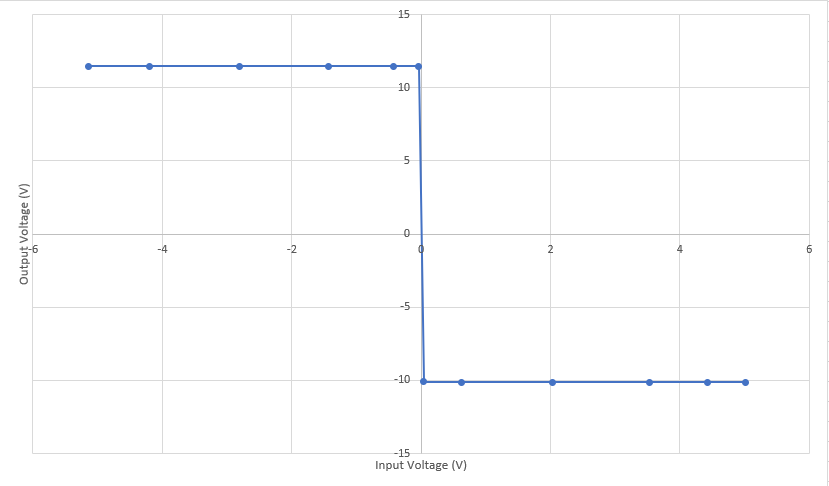
\includegraphics[scale = 0.7]{OPAMP Apps/invwothres.png}
\end{center}
\begin{center}
    \textbf{Inverting Without Threshold}
\end{center}
\clearpage
\begin{center}
    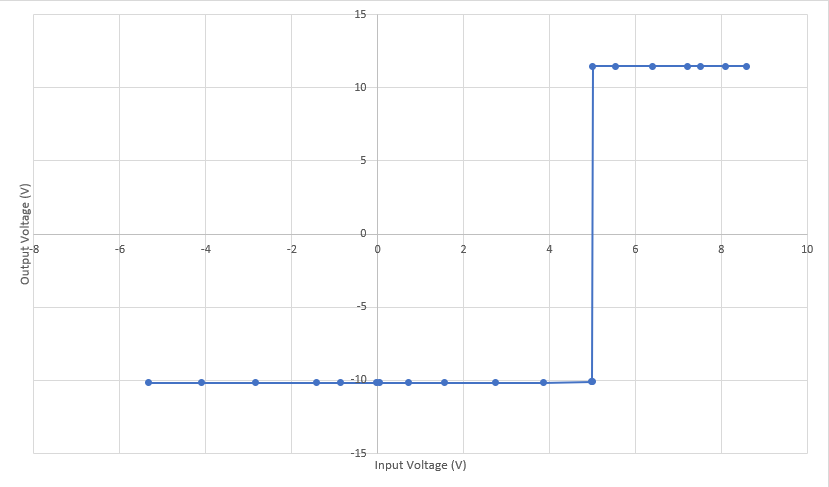
\includegraphics[scale = 0.7]{OPAMP Apps/noninvthres.png}
\end{center}
\begin{center}
    \textbf{Non-inverting With Threshold}
\end{center}
\begin{center}
    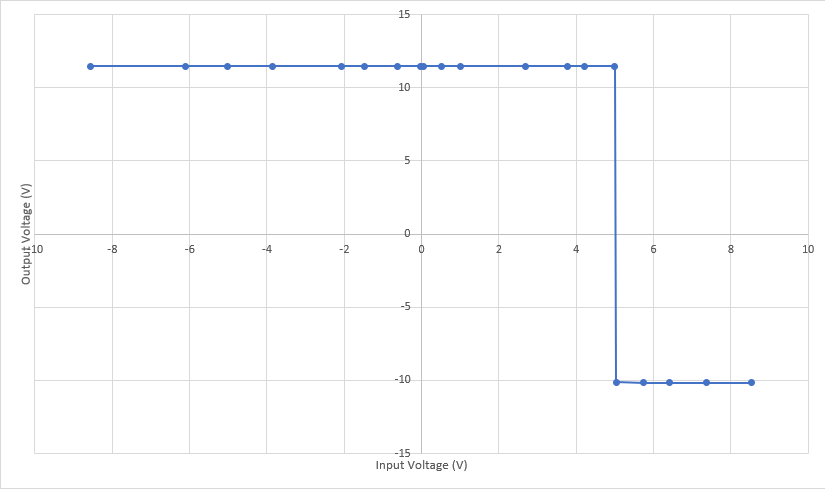
\includegraphics[scale = 0.7]{OPAMP Apps/invthres.png}
\end{center}
\begin{center}
    \textbf{Inverting With Threshold}
\end{center}
\clearpage
\begin{center}
    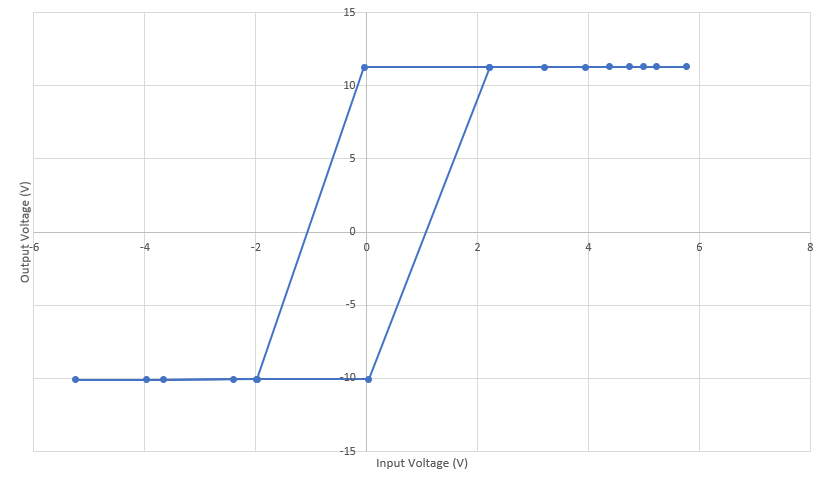
\includegraphics[scale = 0.7]{OPAMP Apps/schmitttrigger.png}
\end{center}
\begin{center}
    \textbf{\emph{Hysteresis}-like loop formed by Schmitt Trigger}
\end{center}
\section{Results}
\begin{enumerate}
    \item The inverting comparator circuit without threshold gives two saturation values, where the output signal has the opposite sign as that of the input signal. The polarity changes at \SI{0}{\volt}. These saturation values are close to $V_{++}$ and $V_{--}$.
    \item The non-inverting comparator circuit without threshold gives two saturation values, where the output signal has the same sign as that of the input signal. The polarity changes at \SI{0}{\volt}. These saturation values are close to $V_{++}$ and $V_{--}$.
    \item The inverting comparator circuit with threshold gives two saturation values where the output signal has the opposite sign as that of the input signal. The polarity changes at $V_{Th} = \SI{5.00}{\volt}$. These saturation values are close to $V_{++}$ and $V_{--}$.
    \item The non-inverting comparator circuit with threshold gives two saturation values where the output signal has the same sign as that of the input signal. The polarity changes at $V_{Th} = \SI{5.00}{\volt}$. These saturation values are close to $V_{++}$ and $V_{--}$.
    \item The Schmitt trigger yields a hysteresis-like curve.
\end{enumerate}
\section{Discussions}
\begin{enumerate}
    \item The saturation values (both in positive and negative polarities) are close to bias voltages but are not exactly equal. This can be attributed to noise signals.
    \item The behaviour of these circuits is like switches (binary output) so they can be use in various appliances as the same.
    \item They can find applications in logic gates.
    \item The Schmitt Trigger has a band of operations which is ideal for real world applications where there are minor fluctuations in the input signal. It has more resistance to noise too.
    \item The Schmitt Trigger can also used as alert device in many electronic/electrical devices, for example, a temperature switch.
\end{enumerate}
\section{Error Analysis}
\begin{enumerate}
    \item The Threshold Voltage applied to the Comparator is 5V and the experimental results are very close to, with error within 0.1\%.
\end{enumerate}
\section{Conclusion}
\begin{enumerate}
    \item All results obtained are in accordance to the expectations.
    \item The errors are quite small and are due to elements of the circuit.
    \item We have observed that there is not as sharp a distinction between the upper and lower values.
    \item There is still ambiguity in the threshold region.
    \item But for practical purposes, we have a device which can help in designing circuits with automatic switches.
\end{enumerate}